\documentclass[11pt, a4paper]{article}
\usepackage[paper=a4paper, left=1.5cm, right=1.5cm, bottom=1.5cm, top=1.5cm]{geometry}
%
\usepackage[utf8]{inputenc}
\usepackage[spanish]{babel}

% YO
\usepackage{nameref}% Only if hyperref isn't loaded
\usepackage{subfigure}

\usepackage{caratula/caratula}

\begin{document}

\titulo{\center{Trabajo Práctico 2 \\ Dinámica de intercambio de opinión y el efecto de la generación de opinión en la decisión electoral.
}}
\fecha{\today}
\materia{Simulación de Eventos Discretos}

\integrante{Pedro Rodríguez}{197/12}{pedro3110.jim@gmail.com}
\integrante{Daniel J. Foguelman}{667/06}{dj.foguelman@gmail.com}
\integrante{Hernan Modrow}{767/03}{hmodrow@gmail.com}
% \integrante{Pepe Sánchez}{444/12}{pepe@gmail.com}
% \integrante{Roberto Carlos}{111/10}{roberto@gmail.com}

%Carátula
\maketitle
\newpage

%Indice
\tableofcontents
\newpage

% Demás secciones
%
% \section{Introducción}
% Los procesos de intercambio de opinión, donde por las interacciones interpersonales influyen en la toma de decisiones, tienen amplia aplicación en estudios de comportamiento de las personas como por ejemplo en las ciencias sociales, políticas y económicas. Dichos procesos, son de gran interés para el estudio de procesos electorales en los cuales la opinión pública tiene directa injerencia en la decisión del electorado.

En este trabajo, continuaremos el estudio del impacto de los indecisos y su interacción con otros actores de opinión más fuerte y su consecuente impacto en el resultado de una elección bi-partidista. Extenderemos este trabajo introduciendo nuevos eventos, los shocks de opinión. Estos pueden pensarse como eventos que afectan un conjunto de agentes e influyen su opinión de manera exógena. Estos cambios podrán repercutir fuertemente en su opinión.

Buscamos entonces, analizar el impacto de la influencia de los medios de información y las redes sociales en los indecisos del electorado promedio.


En el trabajo elaborado por Dima et.al encontramos dos premisas (entre otras)  sobre las cuales podemos generar un diferencial en el comportamiento de los agentes.

\begin{itemize}
    \item Las interacciones de las celdas es de a pares y unidireccional, y
    \item el vecindario está definido utilizando el vecindario von Neumann
\end{itemize}

Estas dos premisas limitan el intercambio de opiniones entre celdas alejadas entre sí. Dicho proceso, no refleja cambios de opinión cuando o bien los agentes interactúan en ámbitos nuevos o reciben información de por fuera de su núcleo de interacción.



El objeto de estudio definido por Pina et.al es de una elección entre dos
partidos (por ejemplo, en el ámbito de un ballotage presidencial), sometida a un libre
intercambio de opiniones.
Los estados posibles de un agente, se encuentran en un intervalo de valores definido en el [-3, 3]. Donde los valores de [-3, -1) pertenecen a afinidad por el partido A, los valores entre [-1, 1] denotan que el agente se encuentra en estado de indefinición mientras que los valores en el intervalo (1, 3] son del partido B.
El motivo de esto es que el grado de convicción de los sujetos se encuentra en un espectro que varía a través del tiempo.

La grilla bidimensional de los agentes será de dimensión NxN. Para definir la interacción de cada individuo, se presenta una segunda capa en la grilla la cual contiene información sobre la conectividad de cada persona (Fig. 1a). Cada sujeto modificará su estado en base a la información de la convicción de uno de sus primeros vecinos en las direcciones izquierda, derecha, arriba o abajo. Esto se define en una segunda capa de conectividad que cada determinado intervalo de tiempo genera un valor aleatorio en el rango [1, 4] que define de quien toma la influencia. A intervalos de tiempo de longitud Tau, toda la población recomputa su convicción.



\section{Desarrollo}
Para desarrollar el traductor de \texttt{XMILE} a \texttt{DEVSML}, del cual se habló en la sección anterior, decidimos basarnos en 2 (dos) modelos clásicos implementados en \textit{System Dynamics}. 

Estos modelos son: 
\begin{description}
	\item[Teacup] que modela una taza de café en una habitación, que se enfría progresivamente hasta alcanzar la temperatura ambiente
	\item[SIR] 	que modela una población que sucumbe ante una infección que se propaga en la misma, y posteriormente se va recuperando, hasta que no queda ningún infectado
\end{description}

Mediante el estudio de estos dos modelos, analizamos como los diferentes elementos de cada archivo \texttt{XMILE} pueden ser traducidos a un modelo acoplado en DEVS  de forma tal que esta traducción pueda ser ejecutada. 
Partiendo de un modelo escrito en \texttt{XMILE}, transformandolo en un modelo DEVS con formato \texttt{DEVSML} para luego ejecutarlo utilizando el simulador \textit{CD++}. Finalmente replicando los resultados que se obtienen con simuladores de \textit{System Dynamics}.


A continuación, exponemos cada uno de los modelos mencionados, mencionando cómo nos ayudaron en el desarrollo del traductor. 

Aprovecharemos que el modelo \textit{Teacup} traducido contiene pocos archivos para mostrar el código generado por el traductor. Para la exposición del comportamiento de los otros modelos cuya traducción genera una mayor cantidad de archivos, utilizaremos el lenguage formal típico con que se expresan modelos DEVS.

% (http://pysd.readthedocs.io/en/master/)
En el proceso de investigación realizado en este trabajo, encontramos la herramienta \textit{PySD}\cite{pysd}, que permite simular modelos \textit{Vensim} el lenguaje Python, simplificando de forma considerable el análisis y las corridas de los modelos \texttt{SD} y su comparación con los modelos \textit{CD++} correspondientes efectuados en el TP.

\subsection{Modelo Teacup}
% TODO REVISAR
\subsubsection{Modelo gráfico}
Como se puede observar en la figura \ref{fig:Teacup_sd} el modelo cuenta con 1 (un) \textit{stock} para modelar la temperatura de la taza, que llamamos \textit{Teacup Temperature}, 2 (dos) auxiliares, que en este caso son constantes, pero podrían ser funciones, una para la temperatura del cuarto, (\textit{Room Temperature}, y otra para el tiempo característico, \textit{Characteristic Time}), y un flujo de salida (\textit{outflow}) para la perdida de calor de la taza hacia el cuarto,\textit{Heat Loss to Room}, con origen el \textit{stock} \textit{Teacup Temperature} y destino vacío. 

Las flechas negras indican que el flujo de salida proveniente de \textit{Teacup Temperature} utiliza dicha constantes auxiliares en su función interna para determinar el valor de dicho flujo de salida en cada instante en el tiempo. La flecha azul, indica que dicha función también utiliza el valor del \textit{stock} \textit{Teacup Temperature} para hacer este cálculo. 

\begin{figure}[!h]
\centering
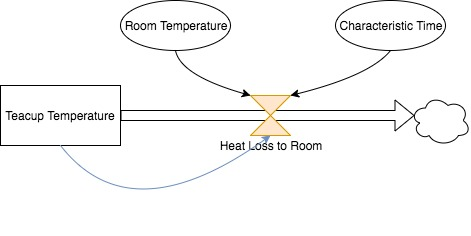
\includegraphics[scale=0.5]{imagenes/Teacup_sd.jpg}
\caption{Modelo \textit{Teacup} expresado en \textit{System Dynamics} en formato gráfico}
\label{fig:Teacup_sd}
\end{figure}

\begin{figure}[!h]
\centering
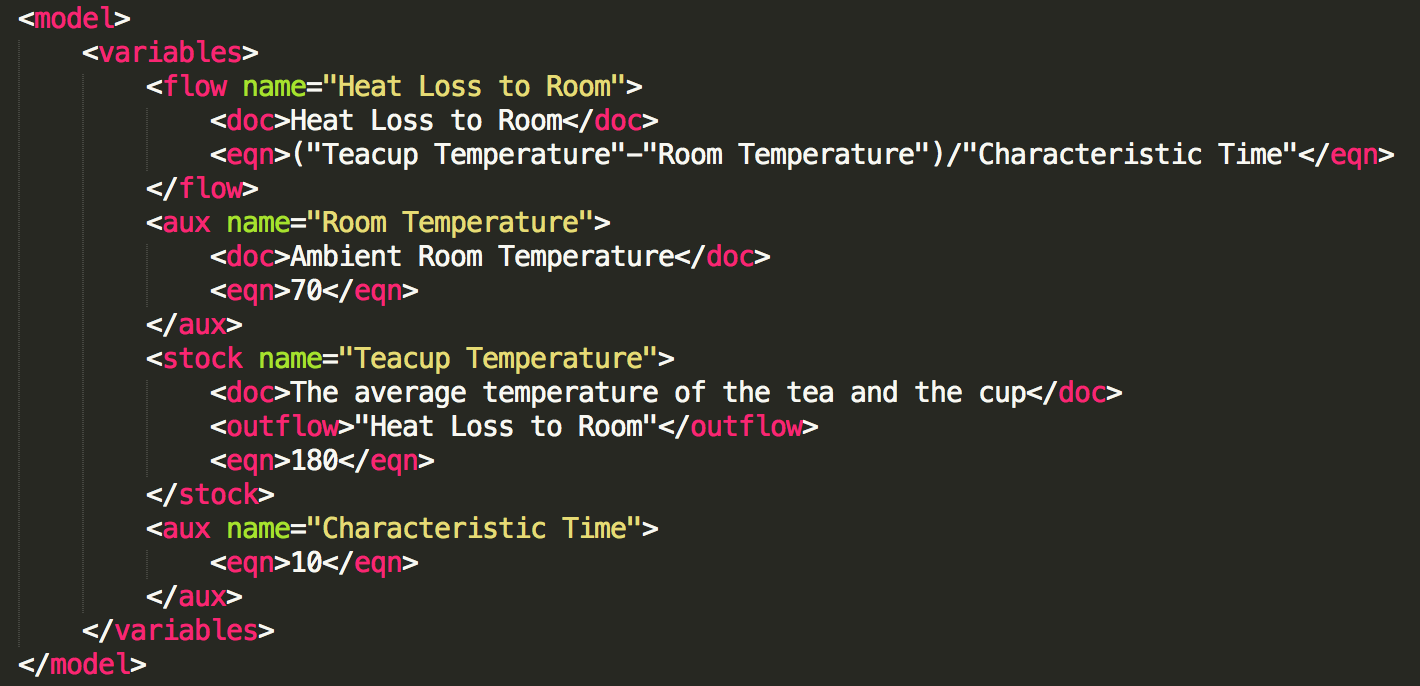
\includegraphics[scale=0.5]{imagenes/teacup_mapeo/Teacup_variables}
\caption{Modelo \textit{Teacup} expresado en \textit{System Dynamics} en formato \texttt{XMILE}}
\label{fig:Teacup_xmile}
\end{figure}

Como se puede observar en la figura \ref{fig:Teacup_xmile}, se utilizan distintos \textit{tags} para los elementos de \textit{System Dynamics}, uno para los flujos de entrada (\textit{inflows}) y salida (\textit{outflows}) (el \textit{tag} \textbf{flow} en el archivo \texttt{XMILE}), otro para las constantes auxiliares (el  \textit{tag} \textbf{aux}) y otro para los stocks (el \textit{tag} \textit{stock}). 

Asimismo, en cada flujo, se utiliza un \textit{tag} \textbf{eqn} en archivo \texttt{XMILE} para mostrar la función utilizada por dicho \textit{flow} (que puede ser tanto de \textit{input} ó \textit{output}) para agregarle o quitarle unidades respectivamente al \textit{stock} sobre el que operan. 

Observamos que en los stocks y variables auxiliares se utiliza el \textit{tag} \textbf{eqn} para mostrar el valor inicial de dicho \textit{stock} ó variable auxiliar. En este caso, las variables auxiliares son todas constantes, con lo cuál en el \textit{tag} \textbf{eqn} contiene el valor que se mantendrá igual durante toda la simulación.

A partir de estas observaciones, decidimos representar este mismo modelo en el formalismo DEVS, de la forma en que se muestra en el diagrama de la figura \ref{fig:Teacup_devs_flattened}

\begin{figure}[!h]
\centering
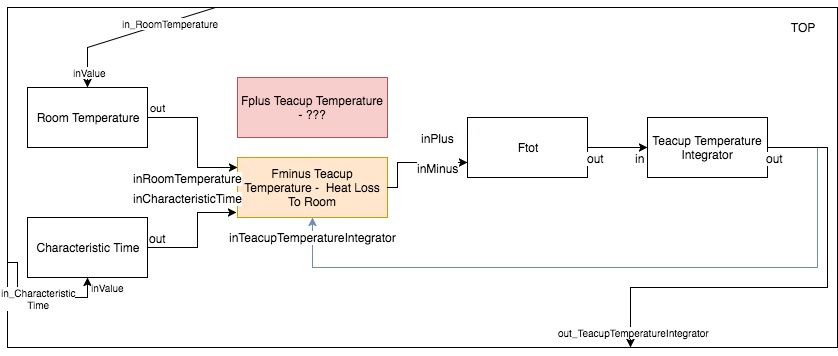
\includegraphics[scale=0.5]{imagenes/Teacup_devs_flattened}
\caption{Modelo \textit{Teacup} expresado en DEVS en formato gráfico}
\label{fig:Teacup_devs_flattened}
\end{figure}

En el diagrama de la figura \ref{fig:Teacup_devs_flattened} se puede observar lo siguiente: el \textit{stock} se corresponde en el modelo DEVS con dos atómicos.

\begin{itemize}
	\item Un integrador QSS1 de nombre \textit{"Teacup Temperature Integrator"} (\texttt{utilizamo el nombre del \textit{stock} más la palabra \textit{Integrator}})
	\item Un atómico Ftot que determina la variación de unidades que tendrá dicho \textit{stock}, utilizando todos los \textit{inflows} y \textit{outflows} que operan sobre dicho \textit{stock} ($\sum inflows - \sum outflows $). Los \textit{inflows} se conectarán al puerto \texttt{inPlus} y los \textit{outflows} al \texttt{inMinus}. 
\end{itemize}

Por otro lado, a cada flujo (en este caso \textit{Heat Loss to Room} se corresponde con dos atómicos, uno representando el flujo de entrada (\textit{inflow}) y otro la flujo de salida (\textit{outflow}). Esto es para darle mejor legibilidad al modelo.

Decidimos nombrarlo de esta manera, en el caso de un \textit{outflow} concatenando \textit{Fminus} el nombre del \textit{stock} sobre el cual opera y el nombre del flujo, en el caso del modelo \textit{Teacup} \textit{Fminus Teacup Temperature Heat Loss to Room}.

En el caso de un \textit{inflow}, el nombre es igual salvo que reemplazamos \textit{Fminus} por \textit{Fplus}. En el ejemplo de la figura \ref{fig:Teacup_devs_flattened}, el atómico que representa el \textit{inflow} \textit{Heat Loss to Room} de no cumple ninguna función en el modelo DEVS y es por ello que lo marcamos en rojo. 

Finalmente, a los auxiliares (\textit{tag} \textbf{aux}) del modelo \texttt{SD} se corresponde con atómicos en el modelo DEVS. En este caso, los atómicos emitirán un valor constante a través de su puerto out. Dado que los valores de los auxiliares \textit{Room Temperature} y \textit{Characteristic Time} es utilizado por el flujo \textit{Heat Loss to Room} para el calculo del valor de la función en el modelo \texttt{SD}. En el modelo DEVS estos atómicos se conectarán con los correspondientes a los atómicos del flujo (no realizamos las conexiones al atómico correspondiente al \textit{inflow} ya que no es utilizado en el modelo).

También podemos observar en el diagrama del modelo DEVS una línea azul la cual se corresponde con la línea azul del diagrama \ref{fig:Teacup_sd} (en el modelo \texttt{SD} esto es la utilización de \textit{Teacup Temperature} en el calculo de \textit{Heat Loss to Room}). De esta forma, mostramos que el atómico \textit{FminusTeacupTemperature - Heat Loss to Room} utiliza también el \textit{output} del atómico \textit{Teacup Temperature Integrator} para realizar sus cálculos. 

\subsubsection{Múltiples flujos afectando un stock}
Una pregunta que nos hicimos fue, ¿qué pasaría en el caso de que más de un \textit{outflow} operara sobre \textit{Teacup Temperature}?
Decidimos pensar cómo sería la traducción gráfica del siguiente modelo (figura \ref{fig:Teacup_sd_2}). El mismo tiene un segundo o\textit{outflow} que opera sobre el \textit{stock} \textit{Teacup Temperature}, es decir bajando la temperatura de la taza de té, que representa una máquina de enfriamiento (\textit{Cooling Machine} en la literatura), como puede ser por ejemplo un ventilador. El modelo DEVS correspondiente resolvimos debería ser el de la figura \ref{fig:Teacup_devs_flattened_2}. 

Es decir, que se agregan dos atómicos, uno correspondiente al flujo como \textit{inflow} y otro como \textit{outflow}, como en el caso de la temperatura perdido en el ambiente (\textit{flow} \textit{Heat Loss to Room}) sólo el \textit{outflow} tiene conexiones. El atómico \textit{Ftot} ahora tiene un puerto adicional en uso, para la recepción de los valores \textit{FminsuTeacupTemperature - Heat Loss to Room} como parte de los \textit{outflows} que operan sobre el \textit{stock}, recordemos que este atómicos calcula $\sum inflows - \sum outflows $.

\begin{figure}[!h]
\centering
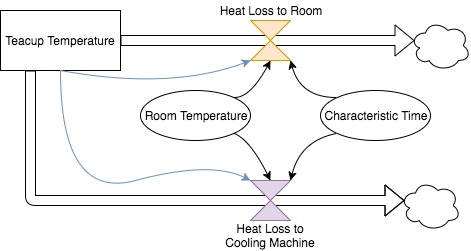
\includegraphics[scale=0.4]{imagenes/Teacup_sd_2}
\caption{Modelo \textit{Teacup} (versión 2) expresado en \texttt{SD} en formato gráfico}
\label{fig:Teacup_sd_2}
\end{figure}

\begin{figure}[!h]
\centering
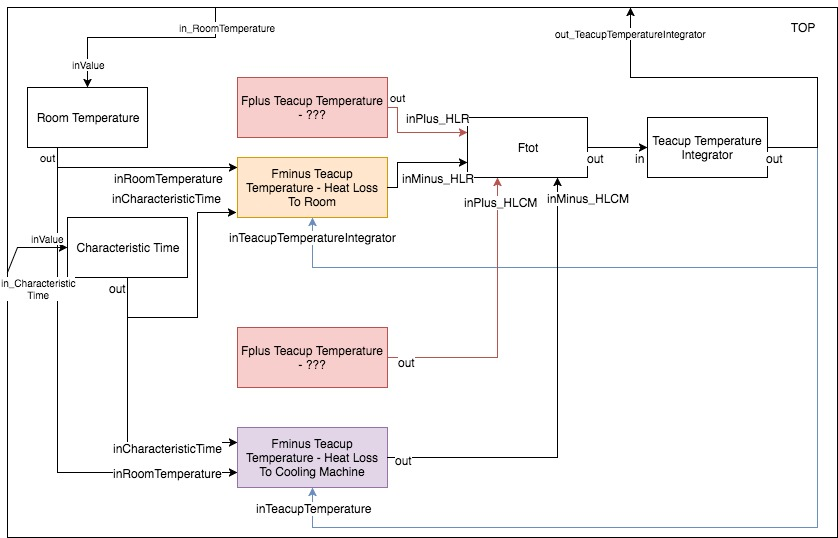
\includegraphics[scale=0.4]{imagenes/Teacup_devs_flattened_2}
\caption{Modelo \textit{Teacup} (versión 2) expresado en DEVS en formato gráfico}
\label{fig:Teacup_devs_flattened_2}
\end{figure}


\subsubsection{El modelo en CD++}
Habiendo generado nuestro modelo DEVS para \textit{Teacup} quisimos ver como sería el mismo en \texttt{CD++}, es decir el archivo \texttt{.ma}, así como también las clases  \texttt{C++} que representan a los atómicos. Ya que estos son los archivos que queremos generar una vez traducido el archivo \texttt{XMILE} a \texttt{DEVSML}.

Por cuestiones de tiempo y para simplificar la implementación, sólo trabajamos con la versión aplanada del modelo. Es decir, no buscaremos generar acoplados alrededor de la dinámica de los \textit{stocks}. Para ver más detalles de como pensamos dichos acoplados ver sección \ref{sssec:cdm}.

\begin{figure}[!h]
\centering
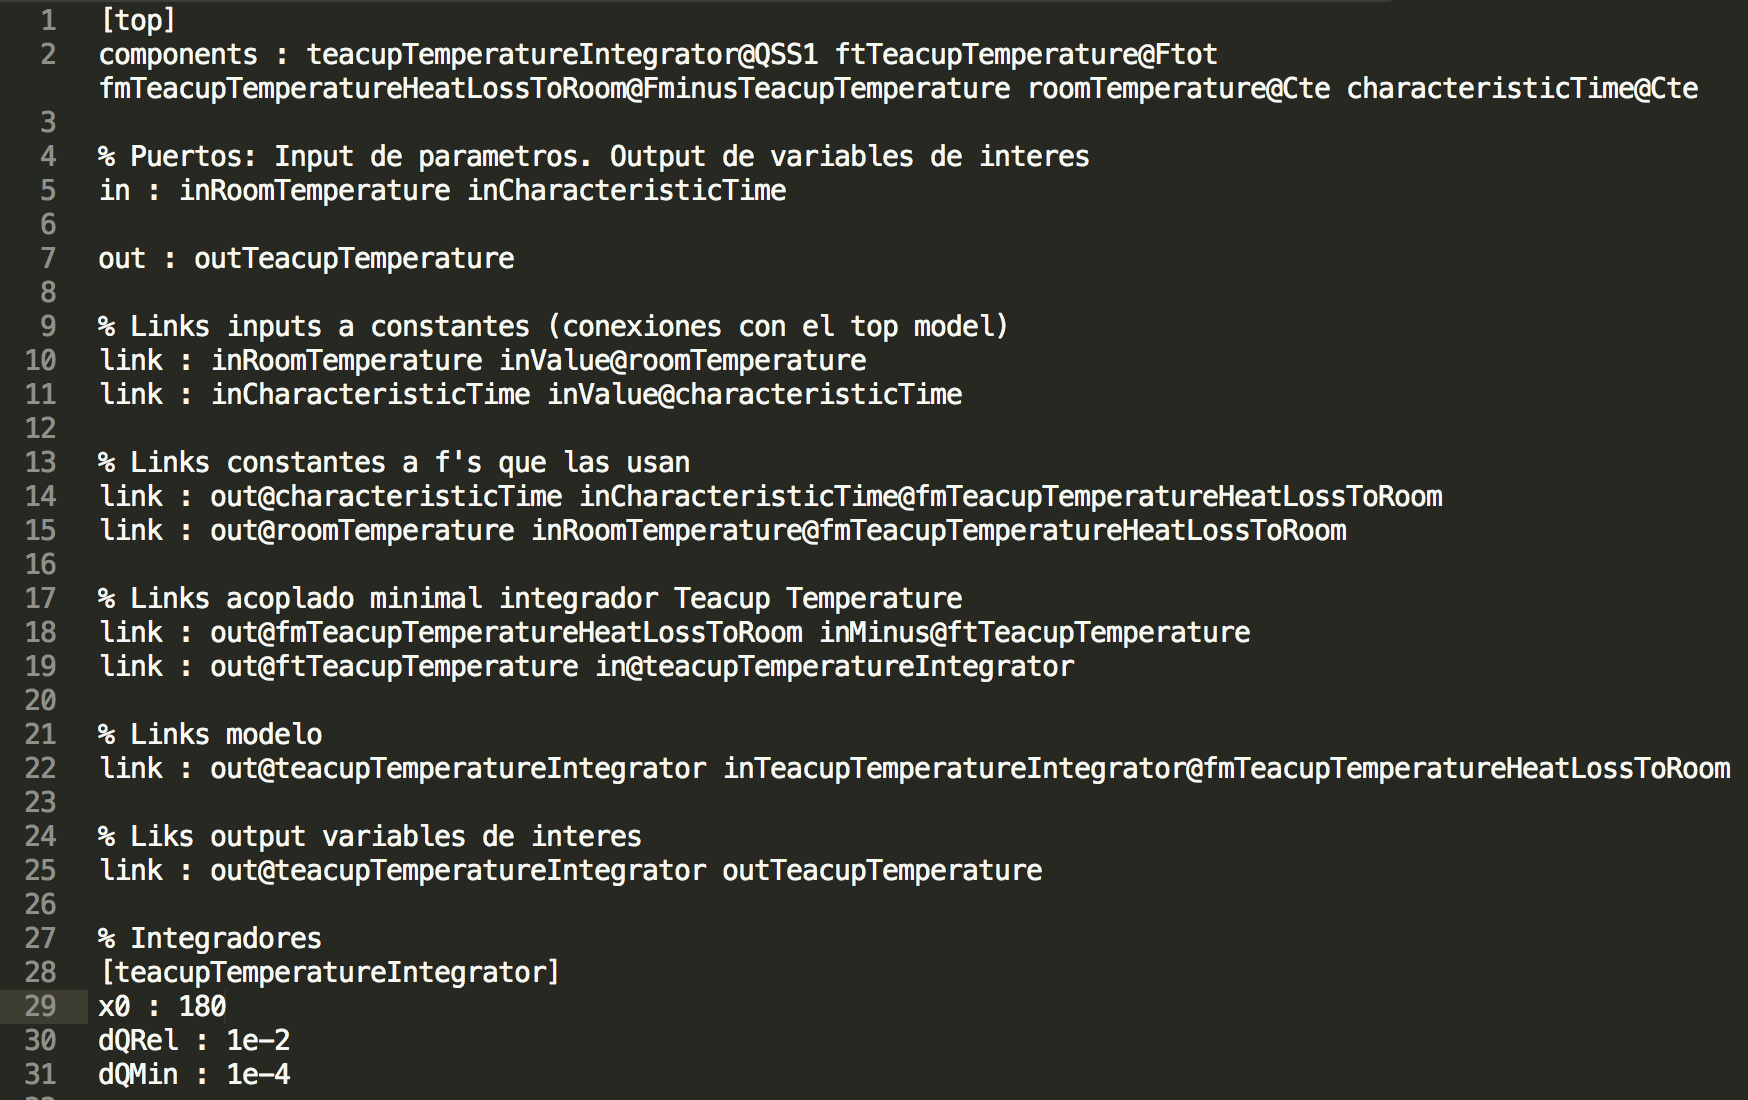
\includegraphics[scale=0.5]{imagenes/teacup_mapeo/Teacup_ma}
\caption{Archivo \texttt{.ma} correspondiente al modelo \textit{Teacup} para simular el modelo en el simulador \textit{CD++}}
\label{fig:Teacup_ma}
\end{figure}

Como se puede observar en la figura \ref{fig:Teacup_ma}, el archivo \texttt{.ma} consta de la definición del componente acoplado que engloba todo el modelo (\texttt{[top]}), la definición de todos los componentes que forman parte de este modelo acoplado (en este caso sólo modelos atómicos), los puertos de entrada y salida, así como los \textit{links} de cada uno de los componentes. En este caso, las entradas son las variables constantes auxiliares y la salida es la única variable de interés del modelo, la temperatura de la taza. 

Si se compara el modelo de la figura \ref{fig:Teacup_devs_flattened} con el archivo \texttt{.ma} de la figura \ref{fig:Teacup_ma}, puede verse una correspondencia entre los descriptos en el archivo con el diagrama DEVS.

Ahora bien, los atómicos utilizados en este modelo tienen cierto comportamiento, por tratarse de \textit{CD++} la implementación será mediante las clases \textit{C++} que sean necesarias. Por lo que vimos, los atómicos que se necesitan implementar, como \textit{Ftot}, \textit{Fmin} o \textit{Fplus}, tienen un comportamiento similar aunque guardan ciertas diferencias (ej: puertos de entrada, función que computan a la salida,etc.) que podríamos tratar de generalizar para poder generar estas clases de manera automática, generando clases específicas para cada atómico que hiciese falta, o crear clases genéricas que permitan generar las diferencias al momentos de instanciar o inicializar los atómicos. 

Nuevamente por cuestiones simplicidad y tiempo, al momento de realizar la implementación, decidimos ir por la primera estrategia, es decir generamos para cada una de las clases necesarias de los atómicos automáticamente sus correspondientes archivos \texttt{.h} y \texttt{.cpp}.

\begin{figure}[!h]
\centering     %%% not \center
\subfigure[Archvo .h]{\label{fig:Teacup_h}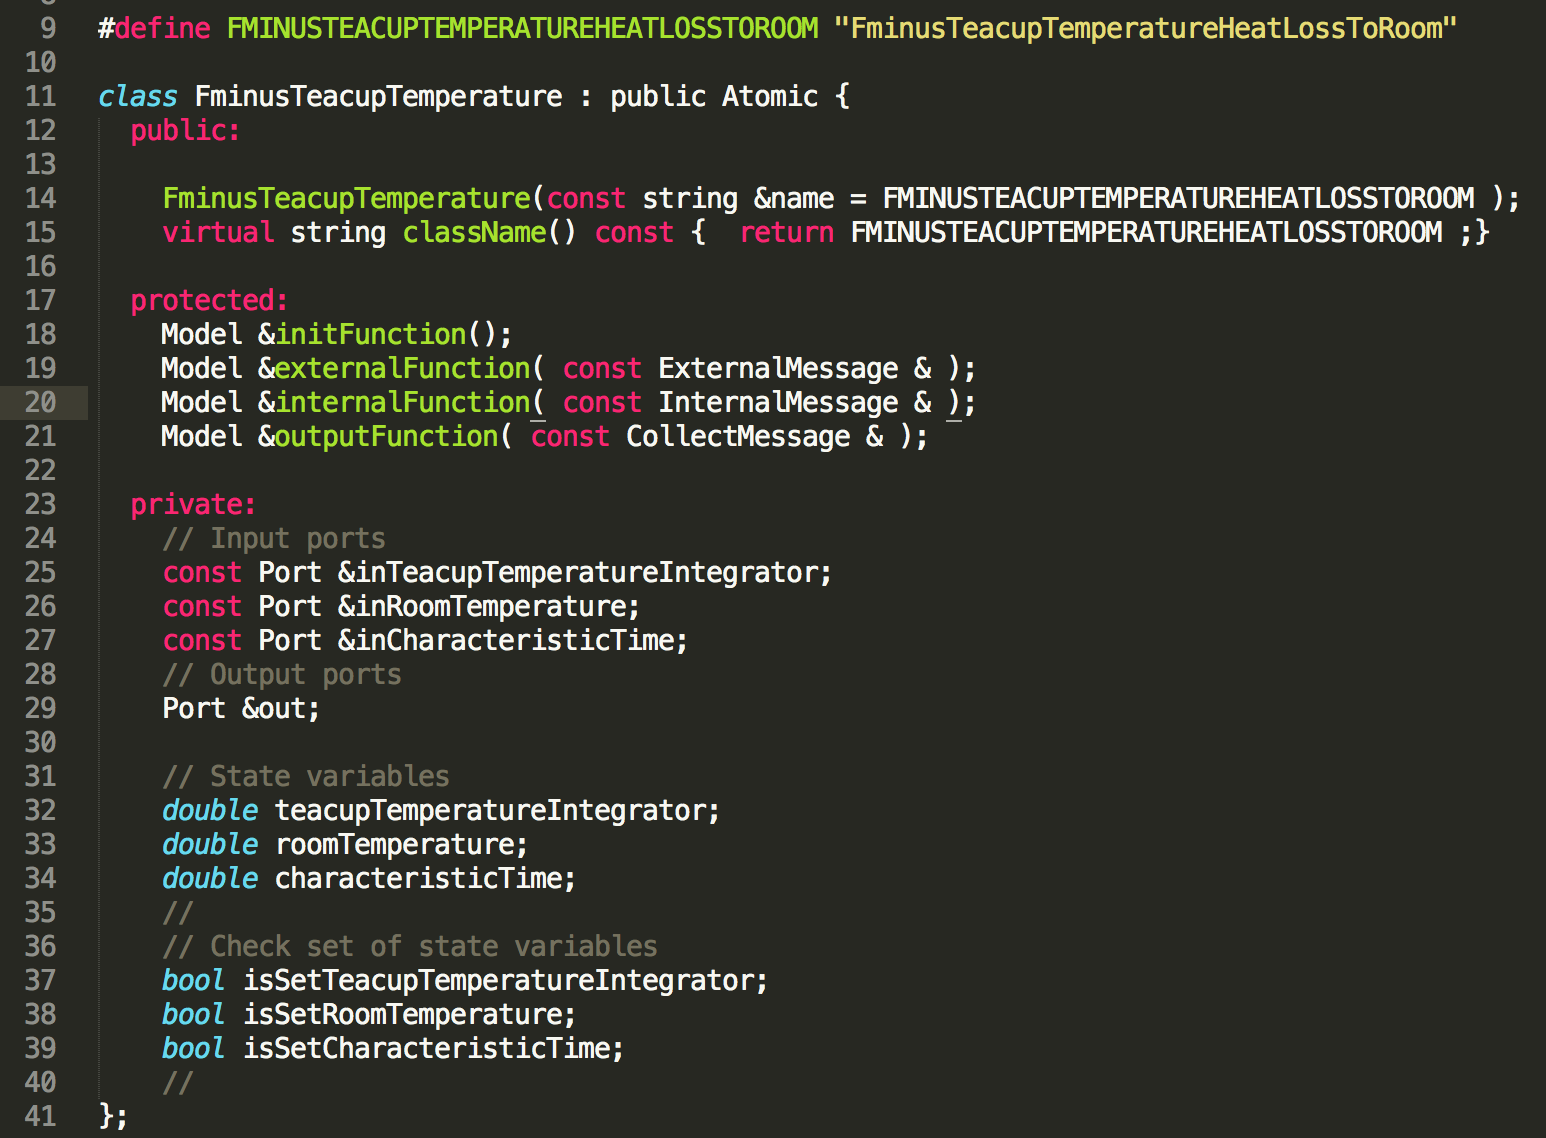
\includegraphics[scale=0.26]{imagenes/teacup_mapeo/Teacup_h}}
\subfigure[Archivo .cpp]{\label{fig:Teacup_hpp}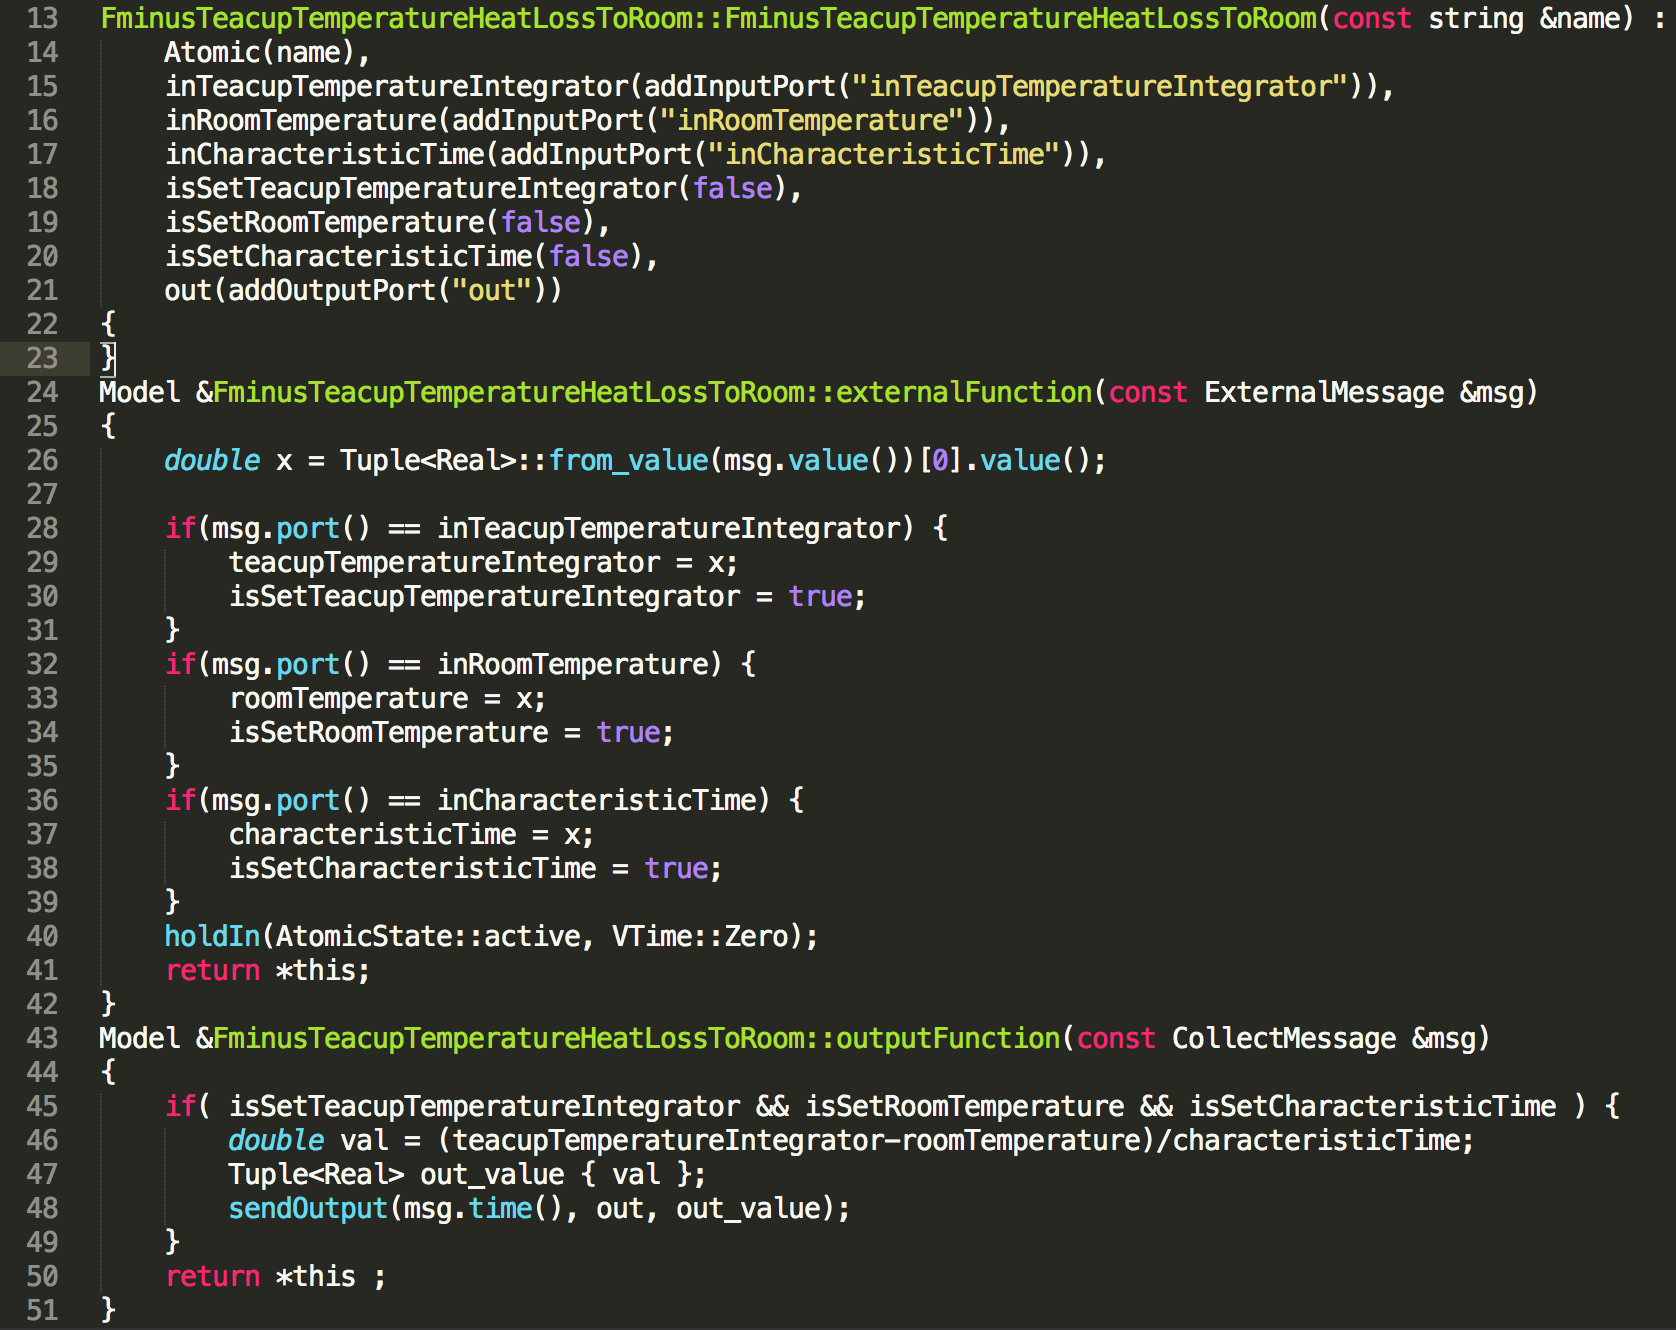
\includegraphics[scale=0.26]{imagenes/teacup_mapeo/Teacup_cpp}}
\caption{Código relevante de los archivos .h y .cpp generados para el atómico FminusTeacupTemperature}
\end{figure}

\begin{figure}[!h]
\centering     %%% not \center
\subfigure[Archvo Ftot.cpp]{\label{fig:Teacup_h}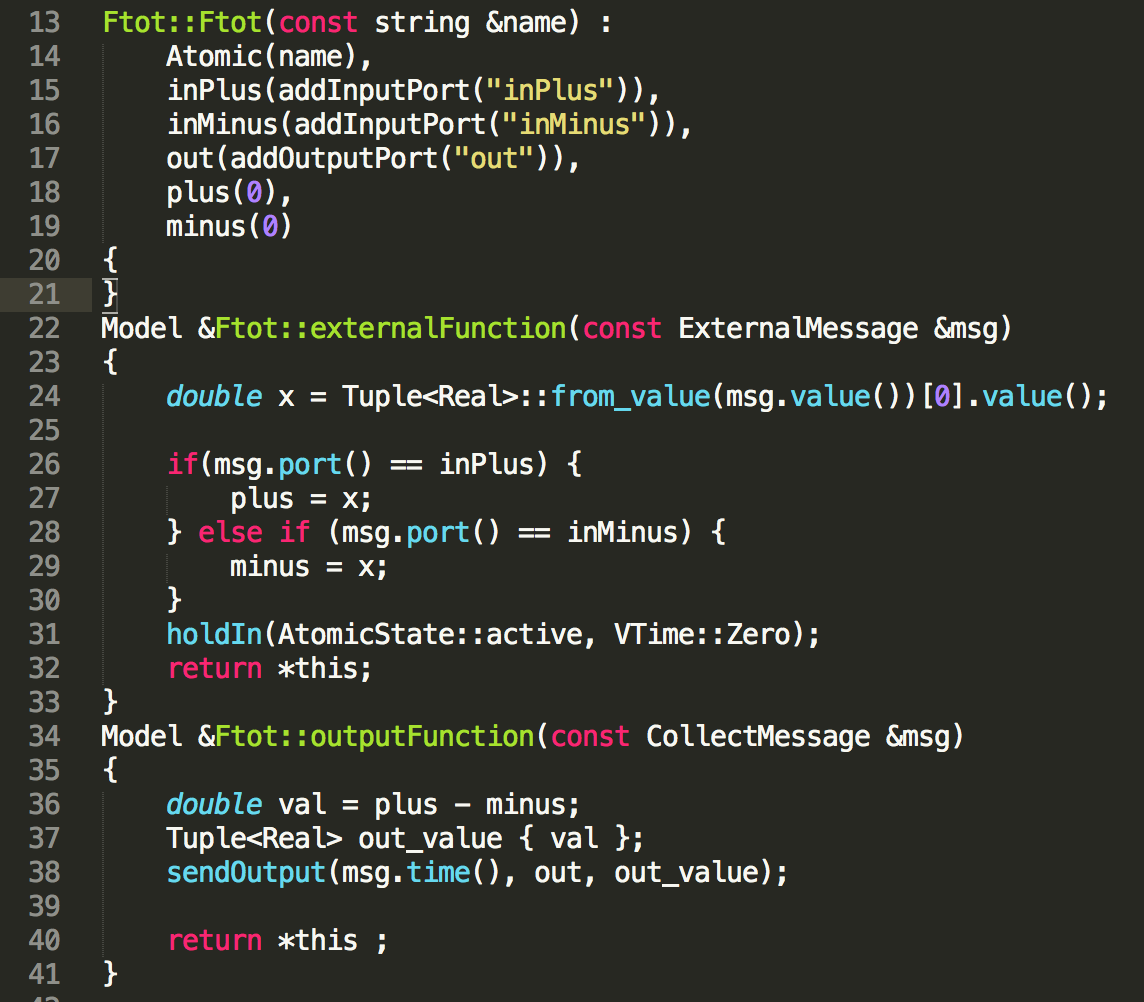
\includegraphics[scale=0.3]{imagenes/gral_mapeo/ftot_cpp}}
\subfigure[Archivo Cte.cpp]{\label{fig:Teacup_hpp}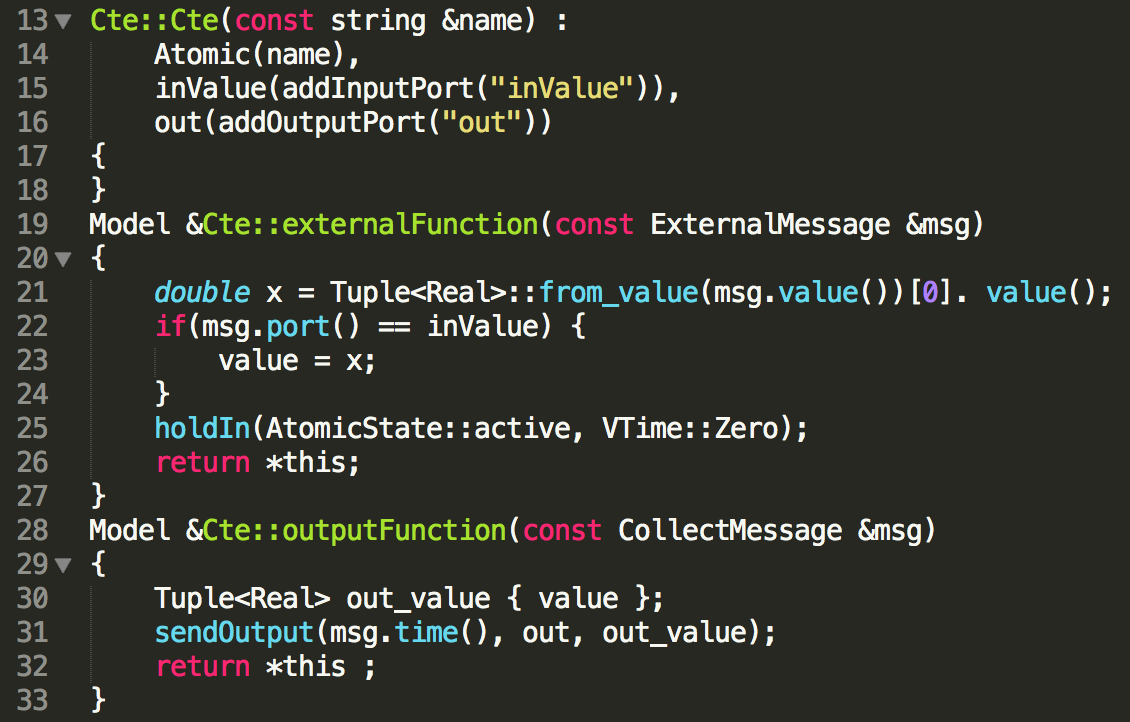
\includegraphics[scale=0.3]{imagenes/gral_mapeo/cte_cpp}}
\caption{Código relevante de los archivos .cpp generados para los atómicos Cte y Ftot}
\end{figure}

\subsubsection{Generación de modelo ejecutable en CD++}
Hemos visto en las secciones anteriores que es posible pasar un modelo en \textit{System Dynamics} a un modelo DEVS, por lo que sería posible generar a partir de un archivo \texttt{XMILE} un archivo \texttt{DEVSML} y a partir de este último generar un archivo \texttt{.ma} y los archivos de necesarios para los atómicos (estos vistos en la sección anterior).

Nos faltaría unicamente revisar el archivo \texttt{DEVSML} del modelo teacup frente al archivo \texttt{.ma} a fin de entender como sería dicha traducción. Como se pueden ver comparando la figura \ref{fig:Teacup_devsml_ports} y \ref{fig:Teacup_devsml_stocks} con la figura \ref{fig:Teacup_ma}, puede verse fácilmente la correspondencia de atómicos, puertos y \textit{links}.

De esta forma, podemos ver que es posible generar las transformaciones necesarias para pasar de un modelo ejecutable especificado en un formalismo de tiempo continuo hacia otro formalismo, de tiempo continuo y eventos discretos.

\begin{figure}[!h]
	\centering     %%% not \center
	\subfigure[Conexiones internas]{\label{fig:Teacup_devsml_internal_connections}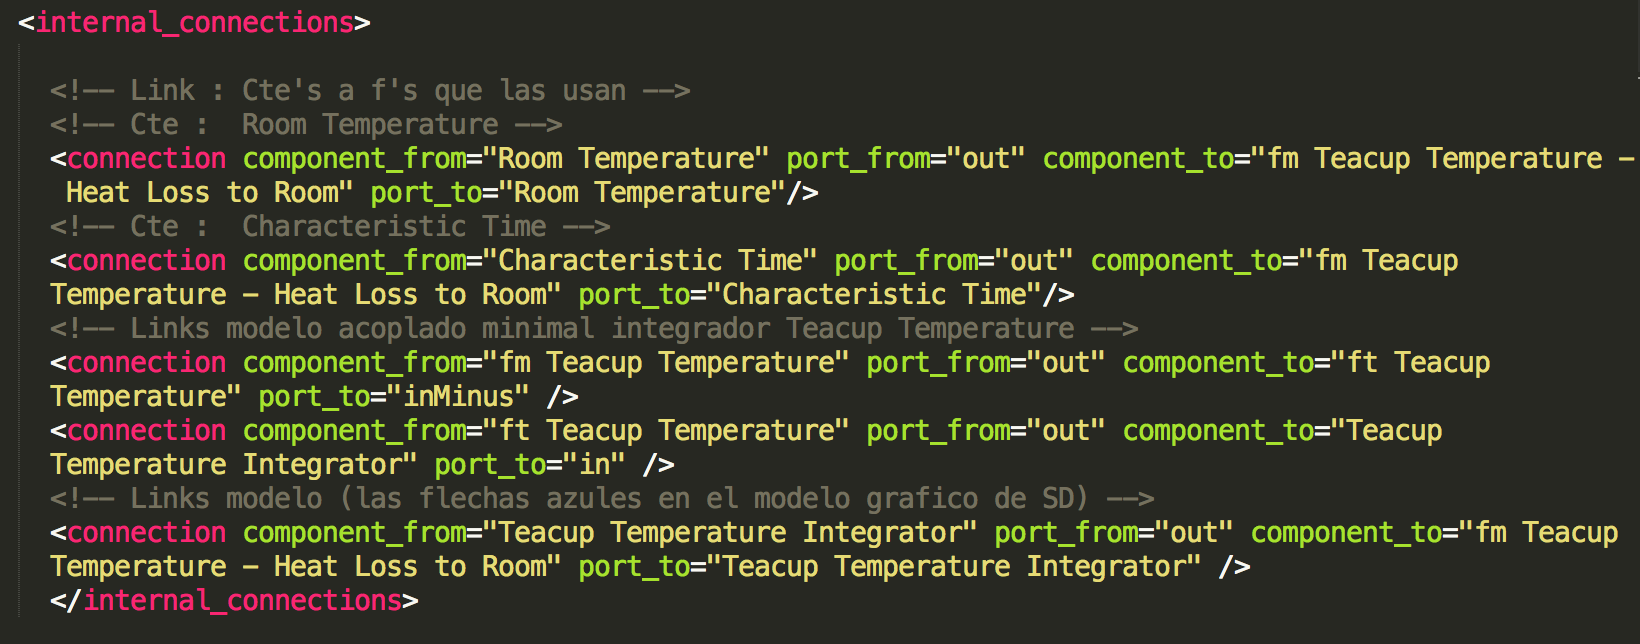
\includegraphics[scale=0.4]{imagenes/teacup_mapeo/Teacup_devsml_internal_connections}}
	\subfigure[Conexiones externas]{\label{fig:Teacup_devsml_external_connections}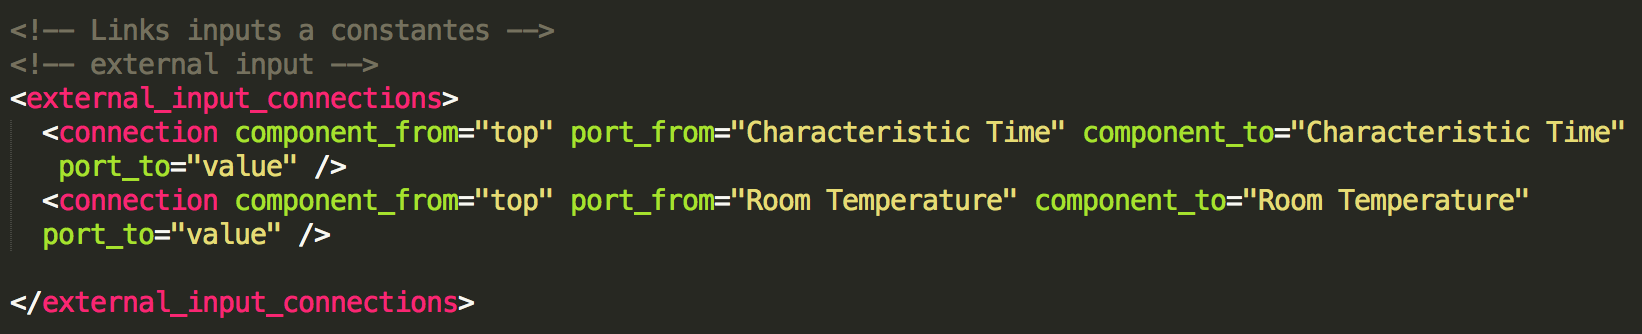
\includegraphics[scale=0.4]{imagenes/teacup_mapeo/Teacup_devsml_external_connections}}
	\subfigure[Puertos de entrada/salida del modelo Top]{\label{fig:Teacup_devsml_ports}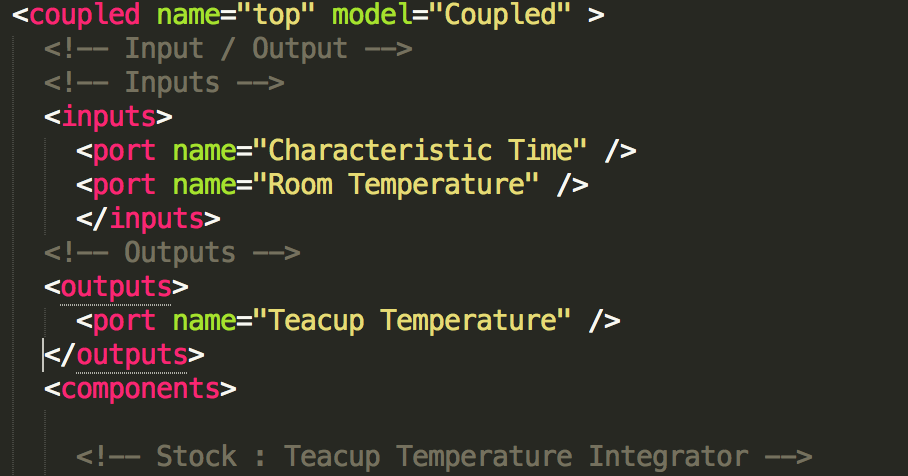
\includegraphics[scale=0.4]{imagenes/teacup_mapeo/Teacup_devsml_ports}}
	\caption{Parte relevante del código .devsml generado por cada conexión y para los puertos del modelo Top}
\end{figure}

\begin{figure}[!h]
\centering     %%% not \center
\subfigure[Atómicos 1-1 para cada Flow]{\label{fig:Teacup_devsml_components}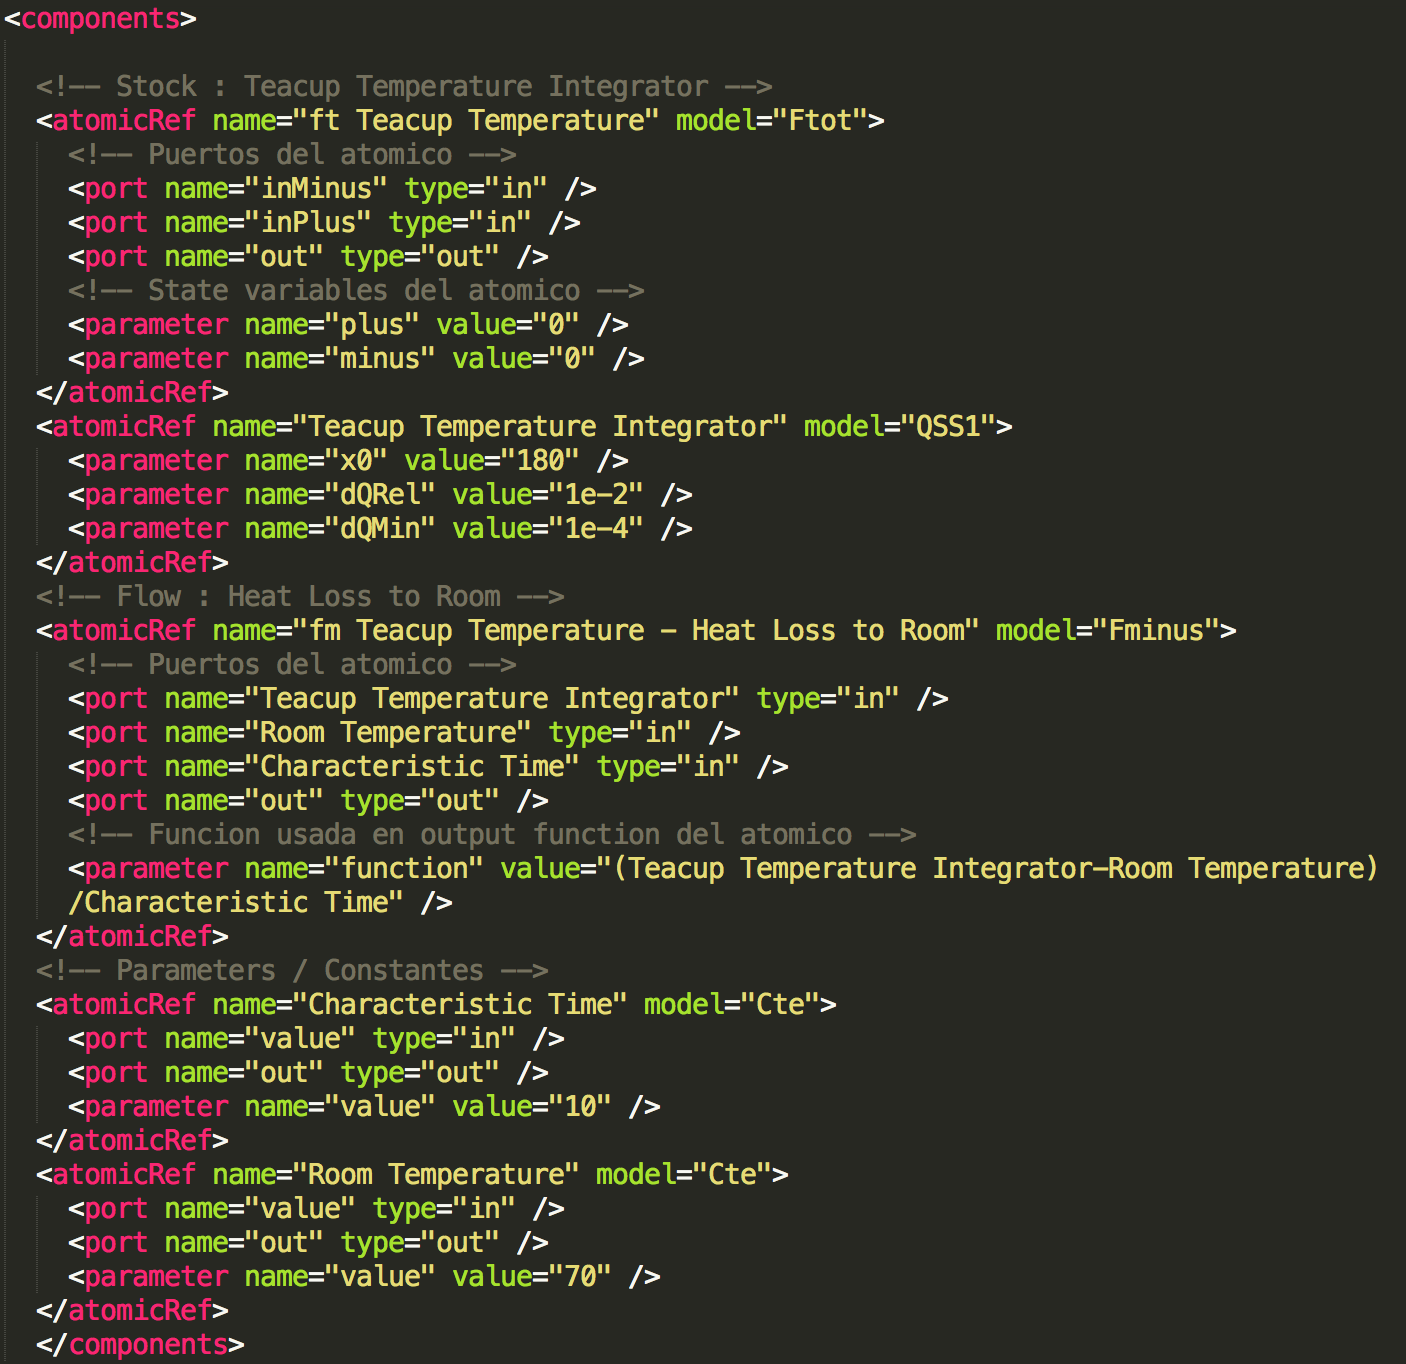
\includegraphics[scale=0.4]{imagenes/teacup_mapeo/Teacup_devsml_components}}
\subfigure[Atómicos 1-1 para cada Stock]{\label{fig:Teacup_devsml_stocks}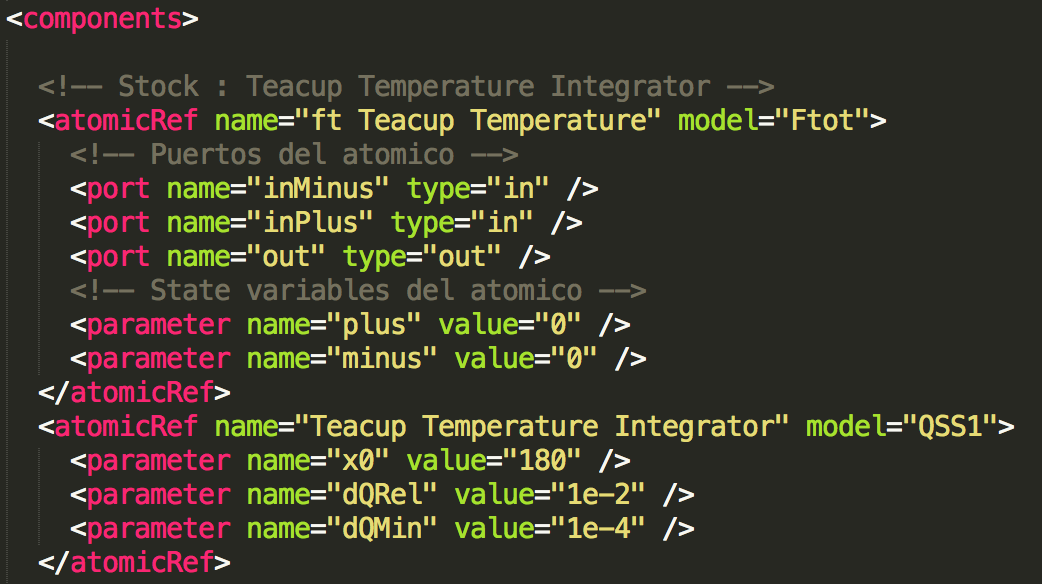
\includegraphics[scale=0.4]{imagenes/teacup_mapeo/Teacup_devsml_stocks}}
\caption{Parte relevante del código .devsml generado por cada Constante, Stock y Flow}
\end{figure}

\pagebreak

\subsubsection{Composibilidad del modelo} \label{sssec:cdm}
¿Es este modelo DEVS obtenido es fácilmente componible con otros? Decidimos ver de que manera era posible modularizar el modelo obtenido, generando un o más acoplados que permitieran componerse con otros.

Si observamos, tanto la temperatura del cuarto como la función características son variables que podrían ser compartidas por otro acoplados de un sistema más complejo, es decir, si una quisiera aislar la dinámica del \textit{stock} podría pensarlos como variables de entrada. Por lo que dicha dinámica, la del \textit{stock}, está encapsulada en el atómico integrador y en el \textit{Ftot} y los flujos que lo modifican, en este caso el atómico \textit{Fminus} que representa el flujo de salida (\textit{outflow}).

Desarrollamos entonces los modelos que se muestra en las figuras \ref{fig:Teacup_devs} y \ref{fig:Teacup_devs_2}, para el modelo original y para la versión con máquina de enfriamiento respectivamente, donde pueden verse los acoplados. 

Todo este análisis nos pareció importante, al momento de desarrollar una primera versión del traductor. Ya que queremos entender de que manera es posible generalizar la forma en que se transformar los modelos \texttt{SD} a modelos DEVS y que además pueda escalar y ser utilizado en modelos más complejos. 

\begin{figure}[!h]
	\centering
	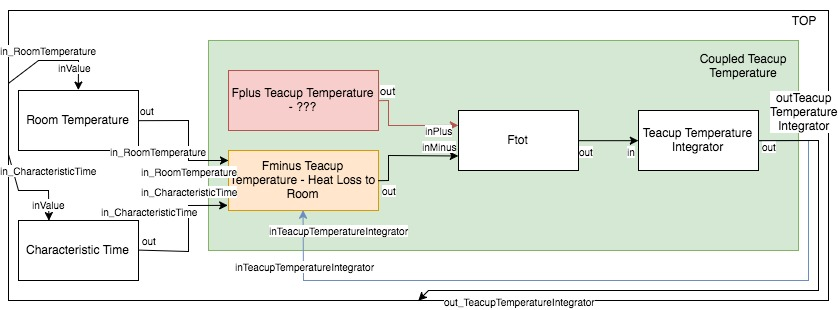
\includegraphics[scale=0.35]{imagenes/Teacup_devs}
	\caption{Modelo \textit{Teacup} expresado en DEVS en formato gráfico utilizando varios niveles de acoplamiento}
	\label{fig:Teacup_devs}
\end{figure}
\begin{figure}[!h]
	\centering
	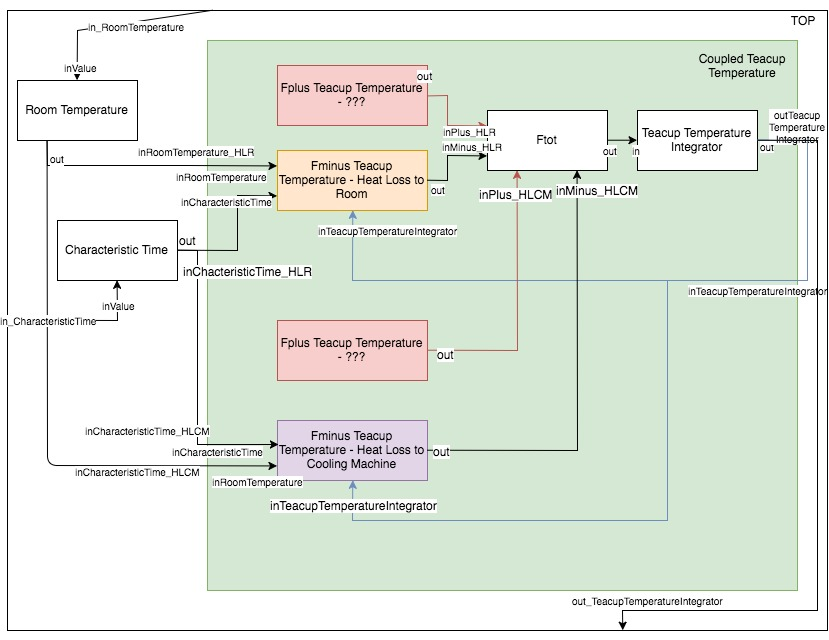
\includegraphics[scale=0.35]{imagenes/Teacup_devs_2}
	\caption{Modelo \textit{Teacup} (versión 2) expresado en DEVS en formato gráfico utilizando varios niveles de acoplamiento}
	\label{fig:Teacup_devs_2}
\end{figure}
% TODO

\subsection{Modelo Teacup}
% TODO Extender el algoritmo
A continuación, y basándonos en lo aprendido durante la construcción del traductor para el modelo \textit{Teacup}, detallaremos un algoritmo inicial y muy básico que pensamos debería servir para traducir archivos \texttt{XMILE} a \texttt{DEVSML}, a partir de la captura de toda la información relevante contenida en el archivo \texttt{XMILE}.

Como mencionamos anteriormente, en esta versión inicial, nos restringimos a traducir a modelos DEVS aplanados solamente (contenidos dentro de un único acoplado). De esta manera, se simplifica la implementación del traductor. Además de esto, restringimos a archivos \texttt{XMILE} que también estén aplanados, es decir, sin submodulos.

Dividiremos la explicación del algoritmo en partes, para entender las figuras \ref{fig:Teacup_devsml_components}, \ref{fig:Teacup_devsml_stocks}, \ref{fig:Teacup_devsml_internal_connections}, \ref{fig:Teacup_devsml_external_connections} y \ref{fig:Teacup_devsml_ports}, explicando como cada una de estas se corresponde con las líneas del archivo \texttt{.ma} expuesto en la figura \ref{fig:Teacup_ma}.

El algoritmo consta de los siguientes pasos:
\begin{itemize}
	\item Por cada \textit{flujo} $F_{i}(S_n,S_m)$ (\textit{flujo} $i$ del \textit{stock} $S_n$ hacia el \textit{stock} $S_m$) se generan los \textit{atómicos DEVS} $F_{minus_{(i)}}(S_n)$ y $F_{plus_{(i)}}(S_m)$. Si $S_n$ es vacío, es decir sólo hay un \textit{inflow} a $S_m$, sólo se genera el $F_{plus}$ y si $S_m$ es vacío, en el caso de sólo un \textit{outflow} con origen en $S_n$, sólo se genera el $F_{minus}$ (siempre alguno de los dos va a ser no vacío)

	\item por cada \textit{aux} $A_i$ se genera un \textit{atómico DEVS} $Cte$ de nombre $A_{i}Cte$, que es un atómico que genera un valor constante.

	\item Por cada \textit{stock} $S_n$ se genera un par de \textit{atómicos DEVS}: $F_{tot_{(S_n)}}$ y $S_{i}Integrador$. Luego, se conecta el \textit{output} del primero con el \textit{input} del segundo. También, se establecen las siguientes conexiones: para cada flujo $j$ tal que existe $F_{plus_{(j)}}(S_n)$, se conecta a este $F_{plus}$ a un puerto de entrada de suma del $F_{tot}$, mientras que si existe $F_{minus_{(j)}}(S_n)$, se conecta el $F_{minus}$ a un puerto de entrada de resta del $F_{tot}$.
	
	\item Por cada flujo $F_{i}(S_n,S_m)$ que recibe flechas de los \textit{stocks} $\{ S_1 \dots S_n \}$ (es decir, usa estas variables como parámetros internamente), se establece una conexión entre cada uno de los atómicos $S_{i}Integrador \dots S_{n}Integardor$ y (en caso de existir) $F_{minus_{(i)}}(S_n)$ y $F_{plus_{(i)}}(S_m)$.

	\item Por cada flujo $F_{i}(S_n,S_m)$ que recibe flechas de los \textit{aux} $\{ A_1 \dots A_m \}$, se establece una conexión entre cada uno de los atómicos $A_{i}Cte \dots A_{n}Cte$ y (en caso de existir) $F_{minus_{(i)}}(S_n)$ y $F_{plus_{(i)}}(S_m)$.

\end{itemize}


\subsection{Modelo SIR}
% TODO

A fin de probar el algoritmo propuesto, decidimos probarlo realizando la conversión del modelo \textit{Teacup} de algún modelo adicional, elegimos para ello el modelo epidemiológico \textit{SIR}.

Como puede verse en esta la figura \ref{fig:SIR_sd} este modelo cuenta de tres \textit{stocks}, \textit{Suceptible}, \textit{Infected}, \textit{Recovered}, unidos mediante dos \textit{flows}, de  \textit{Succumbing} y \textit{Recovering}. Las constantes auxiliares en este modelo son la población total (\textit{Total Population}), tasa de transmisión (\textit{Contact Infectivity}) y duración (\textit{Duration}). En violeta se muestran la información de los \textit{stocks} que requieren los flujos para sus calculos.

En la figura \ref{fig:SIR_devs_flattened} muestra el modelo DEVS equivalente. En color azul los atómicos \textit{Fplus} y \textit{Fminus} asociados al flujo \textit{Succumbing}, mientras que en naranja se observan los atómicos \textit{Fplus} y \textit{Fminus} asociados al flujo \textit{Recovering}. 

También puede verse en violeta  las conexiones que requieren los atómicos que representan los flujos de los integradores (que son producto de la traducción de los \textit{stocks}), ya que utilizan estos valores para sus cálculos, tal como se observaba en el modelo original en \textit{System Dynamics} (figura \ref{fig:SIR_sd}). 

En rojo pueden verse los atómicos de los flujos que no son utilizados en el modelo, pero que igualmente dejamos por completitud, a fin de dejar explícito que esos atómicos podrían estar si hubiera un \textit{inflow} o \textit{outflow} que se les corresponda.

Como ya explicamos anteriormente, por simplicidad el algoritmo sólo generará la versión aplanada del modelo DEVS, aunque generamos el esquema del modelo con acoplados que puede verse en la figura \ref{fig:SIR_devs}.


\begin{figure}[!h]
\centering
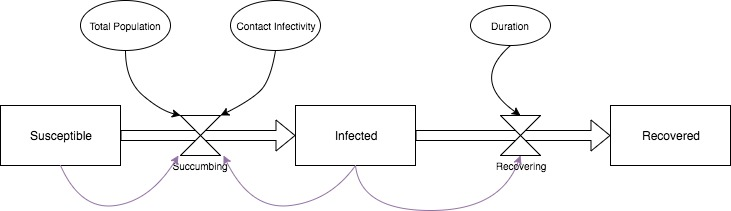
\includegraphics[scale=0.5]{imagenes/SIR_sd.jpg}
\caption{Modelo \textit{SIR} expresado en \textit{System Dynamics} en formato gráfico}
\label{fig:SIR_sd}
\end{figure}
\begin{figure}[!h]
\centering
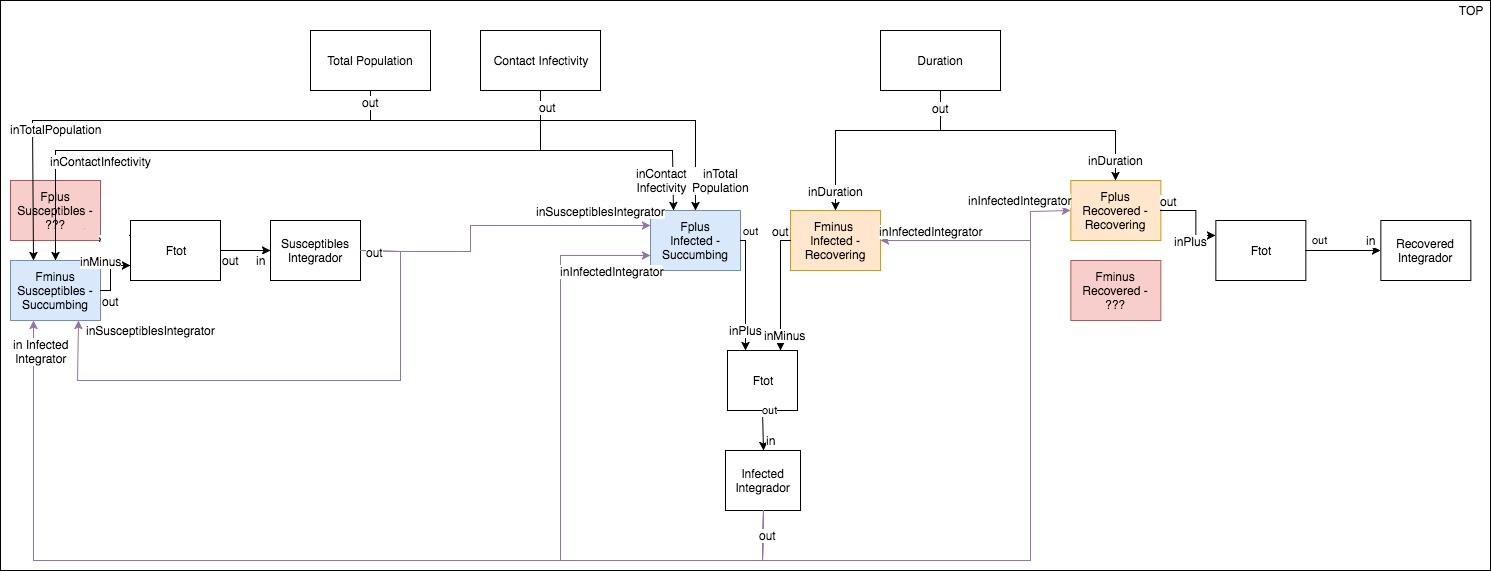
\includegraphics[scale=0.3]{imagenes/SIR_devs_flattened.jpg}
\caption{Modelo \textit{SIR} expresado en DEVS en formato gráfico}
\label{fig:SIR_devs_flattened}
\end{figure}
\begin{figure}[!h]
\centering
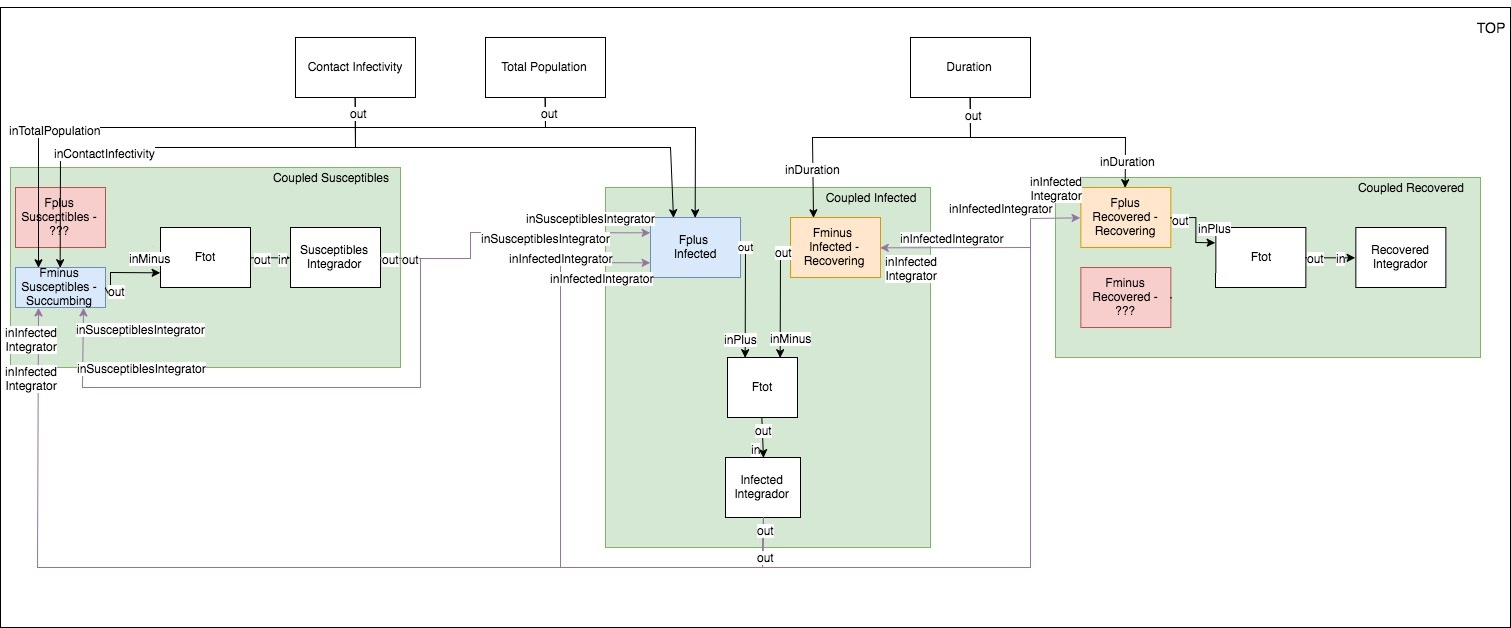
\includegraphics[scale=0.3]{imagenes/SIR_devs.jpg}
\caption{Modelo \textit{SIR} expresado en DEVS en formato gráfico con varios niveles de acoplamiento}
\label{fig:SIR_devs}
\end{figure}
% TODO

% \subsubsection{Generación de modelo ejecutable en CD++}

\subsection{Modelo Lotka-Volterra}
% TODO DECIDIR QUE HACER

\section{Resultados}
%TODO Armar seccion con los graficos 


%
% \section{Conclusiones}
% Durante el desarrollo de este Trabajo Práctico, tuvimos que aprender a utilizar varias herramientas necesarias para la realización del mismo. Entre las más importantes podemos destacar las siguientes:
\begin{itemize}
\item entender el formalismo DEVS y aplicarlo a problemas concretos mediante la utilización del Simulador Avanzado \textit{CD++} desarrollado parcialmente por ex-alumnos de la materia
\item entender el formalismo \textit{System Dynamics} (\texttt{SD}), su capacidad para modelar sistemas de ecuaciones diferenciales continuos, y su relación y punto de contacto con el formalismo DEVS, para poder así reescribir uno modelo de un formalismo al otro
\item tuvimos la necesidad de entender el funcionamiento de los módulos \texttt{QSS}(\textit{Quantized State System}), que utilizamos como integradores en nuestro sistema
\item aplicamos técnicas de \textit{parsing} y transformación de documentos así como también \textit{templates} para simplificar el proceso de traducción de modelos en formato \texttt{XMILE} y formato \texttt{DEVSML} y también para interpretar los \textit{logs} generados por el simulador \textit{CD++}
\item técnicas de visualización para poder comparar eficientemente el \textit{output} generado por el modelo original y por su traducción para los mismos \textit{inputs}
\end{itemize}

A partir de la aplicación de todo lo expuesto más arriba, pudimos ver cómo es posible traducir de forma automática modelos simples (en nuestro caso el modelo \textit{Teacup} y el modelo \textit{SIR}) \textit{System Dynamics} en model DEVS, de forma tal que los resultados de su ejecución para los mismos \textit{inputs} sean cualitativamente iguales, y cuantitativamente casi idénticos.

Con los resultados finales obtenidos, podemos decir que hemos desarrollado exitosamente un traductor simple y básico, que permite traducir de forma automática modelos básico de \textit{System Dynamics} en DEVS, que es un formalismo que al ser basado en eventos discretos, permite incluir en estos modelos variaciones no continuas (que podríamos llamar \textit{eventos}) en el valor de las variables de un modelo en el medio de una simulación de forma natural. De esta forma, la representación de dichos modelos en el formalismo DEVS, permite enriquecer la expresividad del modelo original.
%

\end{document}
